% AI Clinic Defense — Beamer (compile: pdflatex presentation.tex ×2)
\documentclass[aspectratio=169,11pt]{beamer}

\usepackage[T1]{fontenc}
\usepackage{lmodern}
\usepackage{amsmath,amssymb}
\usepackage{booktabs}
\usepackage{graphicx}
\usepackage{xcolor}
\usepackage{hyperref}

% ── Colours (match research report) ──
\definecolor{aivblue}{HTML}{0B3D5C}
\definecolor{aivteal}{HTML}{00A98F}
\definecolor{aivmuted}{HTML}{556677}
\definecolor{aivred}{HTML}{D62728}

\usetheme{Madrid}
\usecolortheme{default}

\setbeamercolor{structure}{fg=aivblue}
\setbeamercolor{frametitle}{bg=aivblue,fg=white}
\setbeamercolor{title}{fg=white,bg=aivblue}
\setbeamercolor{subtitle}{fg=aivmuted}
\setbeamercolor{author}{fg=black}
\setbeamercolor{institute}{fg=aivmuted}
\setbeamercolor{normal text}{fg=black,bg=white}
\setbeamercolor{block title}{bg=aivblue!90,fg=white}
\setbeamercolor{block body}{bg=aivblue!5,fg=black}
\setbeamercolor{alerted text}{fg=aivred}

\setbeamerfont{title}{series=\bfseries,size=\Large}
\setbeamerfont{frametitle}{series=\bfseries}
\setbeamerfont{blocks}{size=\normalsize}

\setbeamertemplate{title page}{
  \vbox{}
  \vfill
  \begingroup
    \centering
    \begin{beamercolorbox}[sep=8pt,center,rounded=true,shadow=true]{title}
      \usebeamerfont{title}\inserttitle\par
      \ifx\insertsubtitle\@empty\else
        \vskip0.25em
        {\usebeamerfont{subtitle}\usebeamercolor[fg]{subtitle}\insertsubtitle\par}
      \fi
    \end{beamercolorbox}
    \vskip1em
    \parbox{0.9\textwidth}{\centering\usebeamerfont{author}\insertauthor}
    \vskip0.6em
    {\usebeamerfont{institute}\insertinstitute\par}
    \vskip0.4em
    {\usebeamerfont{date}\insertdate\par}
    \vskip0.8em
    {\small\textcolor{aivteal}{%
      Environment $\rightarrow$ AI Agent $\rightarrow$ SMC Control $\rightarrow$ Robot}}
  \endgroup
  \vfill
}
\setbeamertemplate{footline}{%
  \hfill\usebeamercolor[fg]{structure}\scriptsize
  PGE5 --- AI Clinic \quad|\quad aivancity\quad|\quad
  \insertframenumber/\inserttotalframenumber\hspace{1em}\vspace{0.5em}
}

\setbeamertemplate{navigation symbols}{}

\newcommand{\highlight}[1]{\textcolor{aivteal}{\textbf{#1}}}

\title[CNN-Adaptive SMC]{CNN-Adaptive Sliding Mode Control\\[0.2em] for Autonomous Differential-Drive Robots}
\subtitle{Under Environmental Uncertainty --- A Digital Twin Approach}
\author[L. Yerra et al.]{%
  Likhita Yerra \and Mohamed Oussama Bouriga \and Ahmed Ben Aissa \and
  Abdellahi El Moustapha \and Thibault Goutorbe}
\institute[aivancity]{%
  PGE5 --- AI Clinic \quad\textbar\quad Supervisor: Prof.\ Vishvjit Thakar\\[0.5em]
  
\includegraphics[height=0.85cm]{../assets/aivancity_logo.png}}
\date{31 August 2026}

\begin{document}

% ─────────────────────────────────────────────
\begin{frame}[plain]
  \titlepage
\end{frame}

% ─────────────────────────────────────────────
\begin{frame}{Outline}
  \tableofcontents
\end{frame}

\section{Introduction}

\begin{frame}{Problem Statement}
  \begin{itemize}
    \item Autonomous mobile robots must track trajectories under \textbf{sensor noise},
          \textbf{external disturbances}, and \textbf{wheel slip}.
    \item Sliding Mode Control (SMC) is robust, but \alert{fixed gains} cannot simultaneously optimise:
    \begin{itemize}
      \item chattering suppression,
      \item tracking accuracy,
      \item disturbance rejection.
    \end{itemize}
    \item Noisy conditions $\Rightarrow$ smoother control; disturbances/slip $\Rightarrow$ aggressive correction.
  \end{itemize}
  \vspace{0.4cm}
  \begin{block}{Research Question}
    \emph{Can a learning-based perception and control pipeline improve SMC adaptability
    for a differential-drive robot under heterogeneous uncertainty?}
  \end{block}
\end{frame}

\begin{frame}{Three Controllers Compared}
  \begin{columns}[T]
    \begin{column}{0.32\textwidth}
      \begin{block}{Classical SMC}
        \begin{itemize}
          \item Fixed gains
          \item Baseline
          \item Struggles under combined uncertainty
        \end{itemize}
      \end{block}
    \end{column}
    \begin{column}{0.32\textwidth}
      \begin{block}{CNN-Adaptive SMC}
        \begin{itemize}
          \item 64$\times$64 map $\rightarrow$ CNN
          \item Scenario $\rightarrow$ preset lookup
          \item Interpretable adaptation
        \end{itemize}
      \end{block}
    \end{column}
    \begin{column}{0.32\textwidth}
      \begin{block}{RL Agent (PPO)}
        \begin{itemize}
          \item Continuous policy
          \item Reward-driven presets
          \item Extension / baseline
        \end{itemize}
      \end{block}
    \end{column}
  \end{columns}
\end{frame}

\section{Methodology}

\begin{frame}{System Architecture}
  \begin{center}
    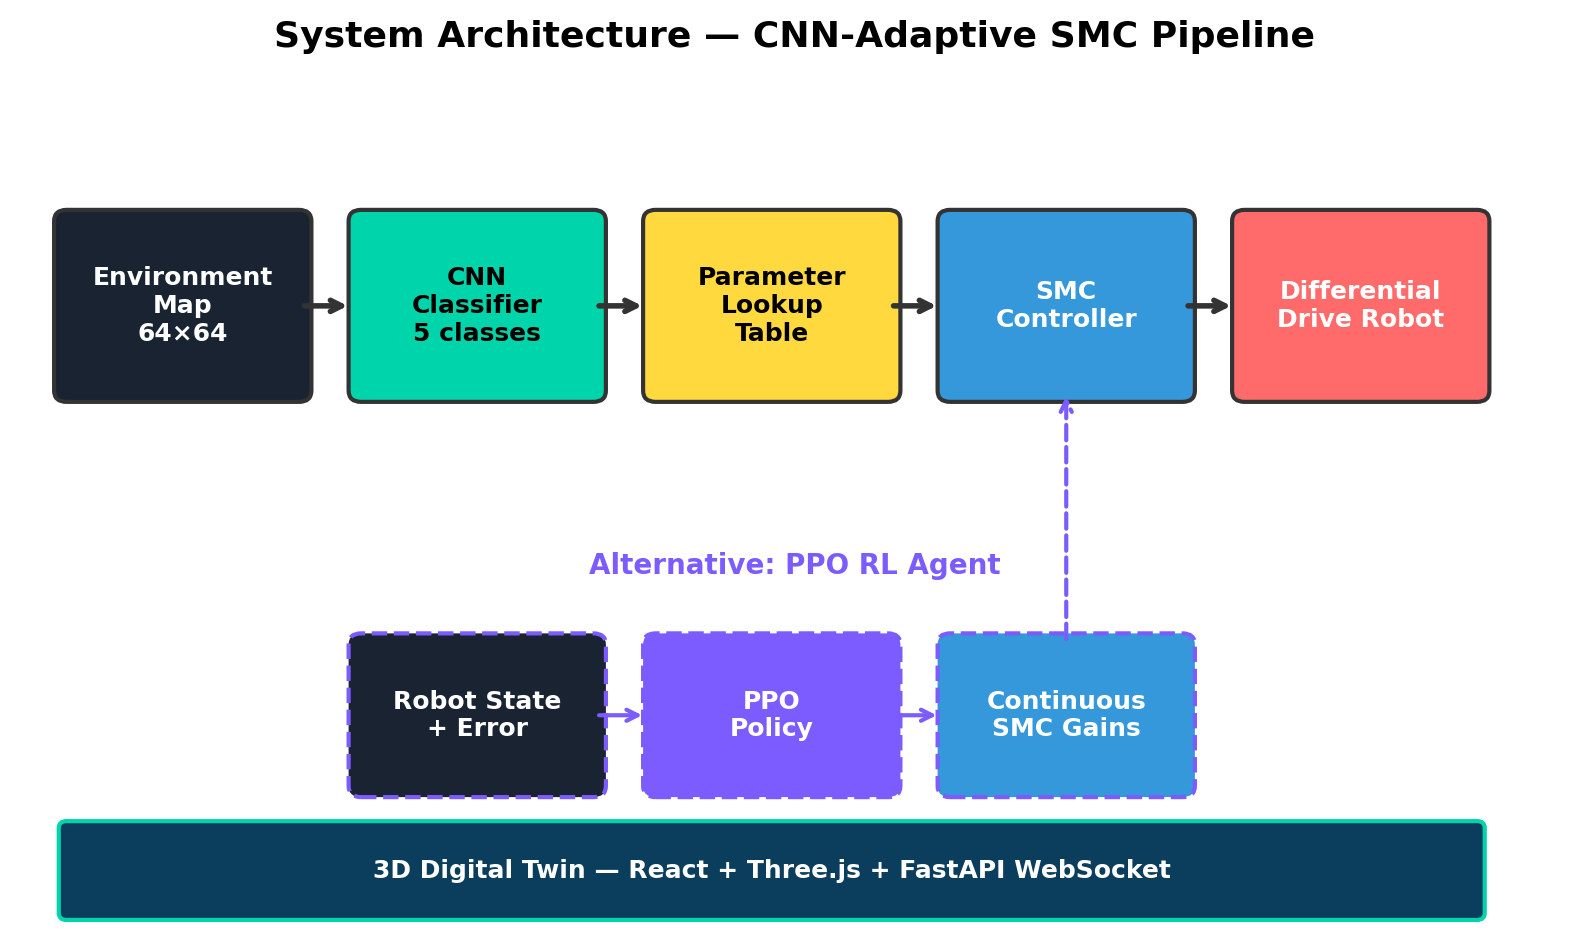
\includegraphics[width=0.92\textwidth]{../assets/figures/fig01_architecture.png}
  \end{center}
  \vspace{-0.2cm}
  {\small CNN-adaptive pipeline (top) and PPO RL alternative (bottom), integrated in the 3D digital twin.}
\end{frame}

\begin{frame}{Robot \& Simulation Model}
  \begin{columns}[T]
    \begin{column}{0.48\textwidth}
      \textbf{Differential-drive unicycle}
      \begin{equation*}
        \dot{x} = v\cos\theta,\quad \dot{y} = v\sin\theta,\quad \dot{\theta} = \omega
      \end{equation*}
      \begin{itemize}
        \item $\Delta t = 0.01$\,s, $L = 0.3$\,m
        \item Reference speed $v_r = 0.3$\,m/s, $T = 20$\,s
        \item Trajectories: straight, circle, S-curve
      \end{itemize}
    \end{column}
    \begin{column}{0.48\textwidth}
      \textbf{Five uncertainty scenarios}
      \begin{table}
        \small
        \begin{tabular}{@{}ll@{}}
          \toprule
          Scenario & Perturbation \\
          \midrule
          Normal & None \\
          Noise & $\sigma_{xy}=0.02$\,m on pose \\
          Disturbance & Push $+0.4$\,m in $y$ at $t=8$\,s \\
          Slip & 30\% velocity loss $t\in[10,14]$\,s \\
          Combined & All three together \\
          \bottomrule
        \end{tabular}
      \end{table}
    \end{column}
  \end{columns}
\end{frame}

\begin{frame}{CNN Environment Classifier}
  \begin{columns}[T]
    \begin{column}{0.52\textwidth}
      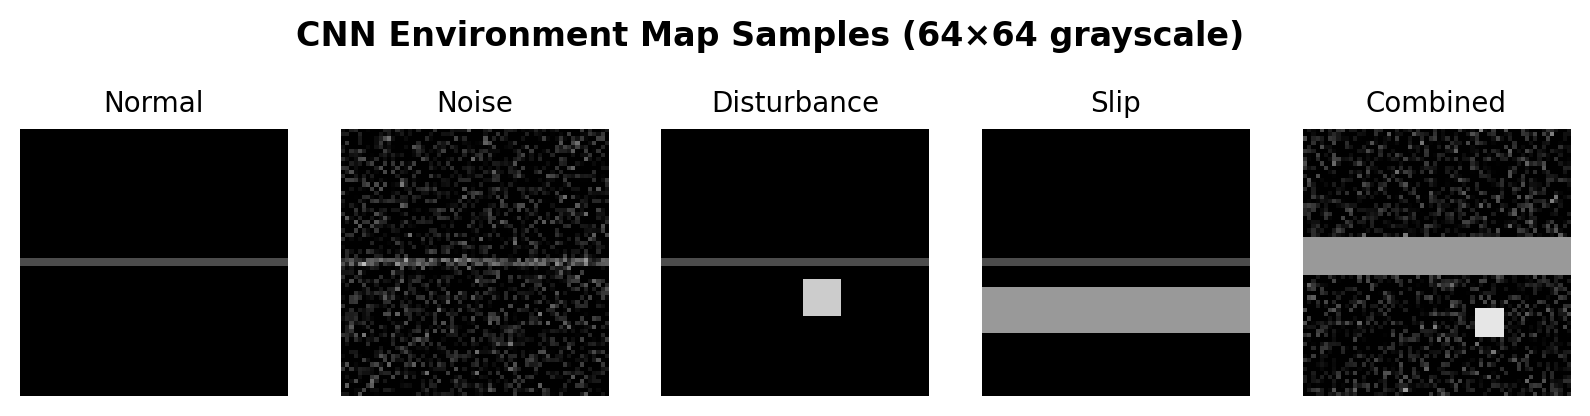
\includegraphics[width=\textwidth]{../assets/figures/fig02_cnn_samples.png}
    \end{column}
    \begin{column}{0.46\textwidth}
      \textbf{EnvironmentCNN} (${\approx}534$k params)
      \begin{itemize}
        \item Input: $1 \times 64 \times 64$ grayscale map
        \item Output: 5 scenario classes
        \item 3 conv blocks + FC + dropout
        \item \highlight{100\%} test acc.\ (simple maps)
        \item \highlight{95.1\%} on realistic maps
        \item Pre-mission classification $\rightarrow$ SMC preset
      \end{itemize}
    \end{column}
  \end{columns}
\end{frame}

\begin{frame}{Adaptive Parameter Selection \& RL Baseline}
  \begin{columns}[T]
    \begin{column}{0.48\textwidth}
      \textbf{CNN-adaptive SMC}
      \begin{itemize}
        \item Map class $\hat{c} \mapsto$ preset $\pi_{\hat{c}}$
        \item Exponential filter: $\pi_k = (1-\beta)\pi_{k-1} + \beta\pi_{\hat{c}}$
        \item Hand-tuned per scenario ($\lambda$, $k$, $\varphi$, $\alpha_\omega$)
        \item Lyapunov UUB analysis grounds design
      \end{itemize}
    \end{column}
    \begin{column}{0.48\textwidth}
      \textbf{PPO RL baseline}
      \begin{itemize}
        \item Gymnasium env + domain randomisation
        \item Obs.: error, error rate, chattering, flags
        \item Action: select preset every 0.2\,s
        \item Reward: $r = -e - 0.05 j_\omega - 0.001|\omega_c|$
        \item 80k training steps
      \end{itemize}
    \end{column}
  \end{columns}
\end{frame}

\section{Results}

\begin{frame}{Headline Results}
  \begin{table}
    \centering
    \begin{tabular}{@{}lcc@{}}
      \toprule
      \textbf{Metric} & \textbf{Improvement} & \textbf{Context} \\
      \midrule
      Chattering index & \highlight{35.7\%} reduction & Sensor noise \\
      Final tracking error & \highlight{14.4\%} improvement & After disturbance \\
      Final tracking error & \highlight{32.7\%} improvement & Wheel slip \\
      CNN vs.\ oracle & 17.9\,mm vs.\ 15.6\,mm & Near-oracle recovery \\
      Realistic-map CNN & \highlight{95.1\%} accuracy & Deployability \\
      \bottomrule
    \end{tabular}
  \end{table}
  \vspace{0.3cm}
  \small\textit{Trade-off: noise scenario widens steady-state error (smoothness vs.\ accuracy per Lyapunov bound).}
\end{frame}

\begin{frame}{Trajectory Comparison --- Combined Scenario}
  \begin{center}
    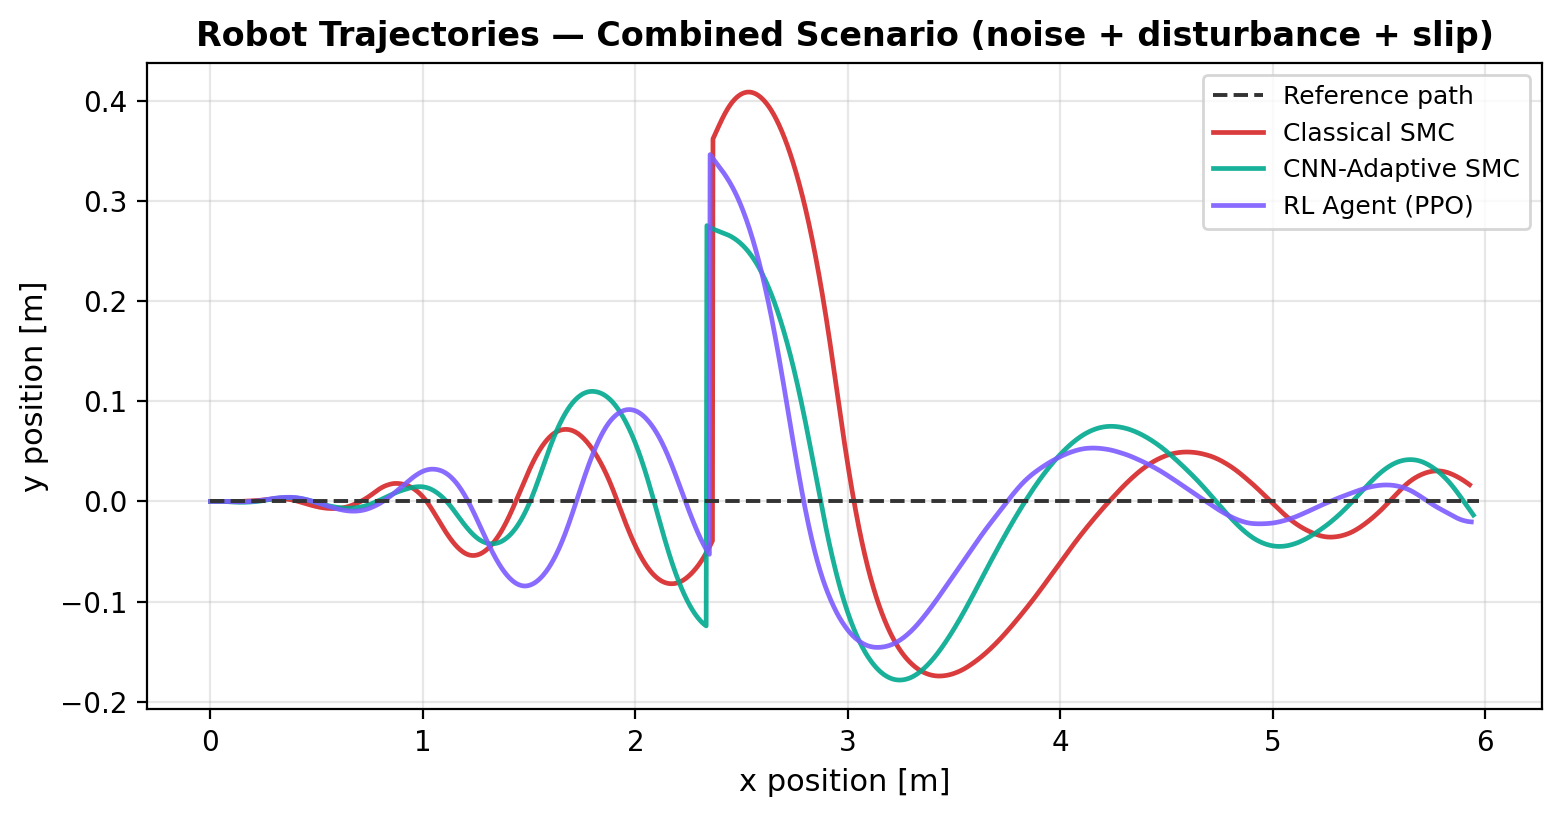
\includegraphics[width=0.82\textwidth]{../assets/figures/fig03_trajectory_comparison.png}
  \end{center}
  \vspace{-0.15cm}
  {\small Impulsive push at $x \approx 2.4$\,m; adaptive controllers recover more tightly to the reference.}
\end{frame}

\begin{frame}{Tracking Error Over Time}
  \begin{center}
    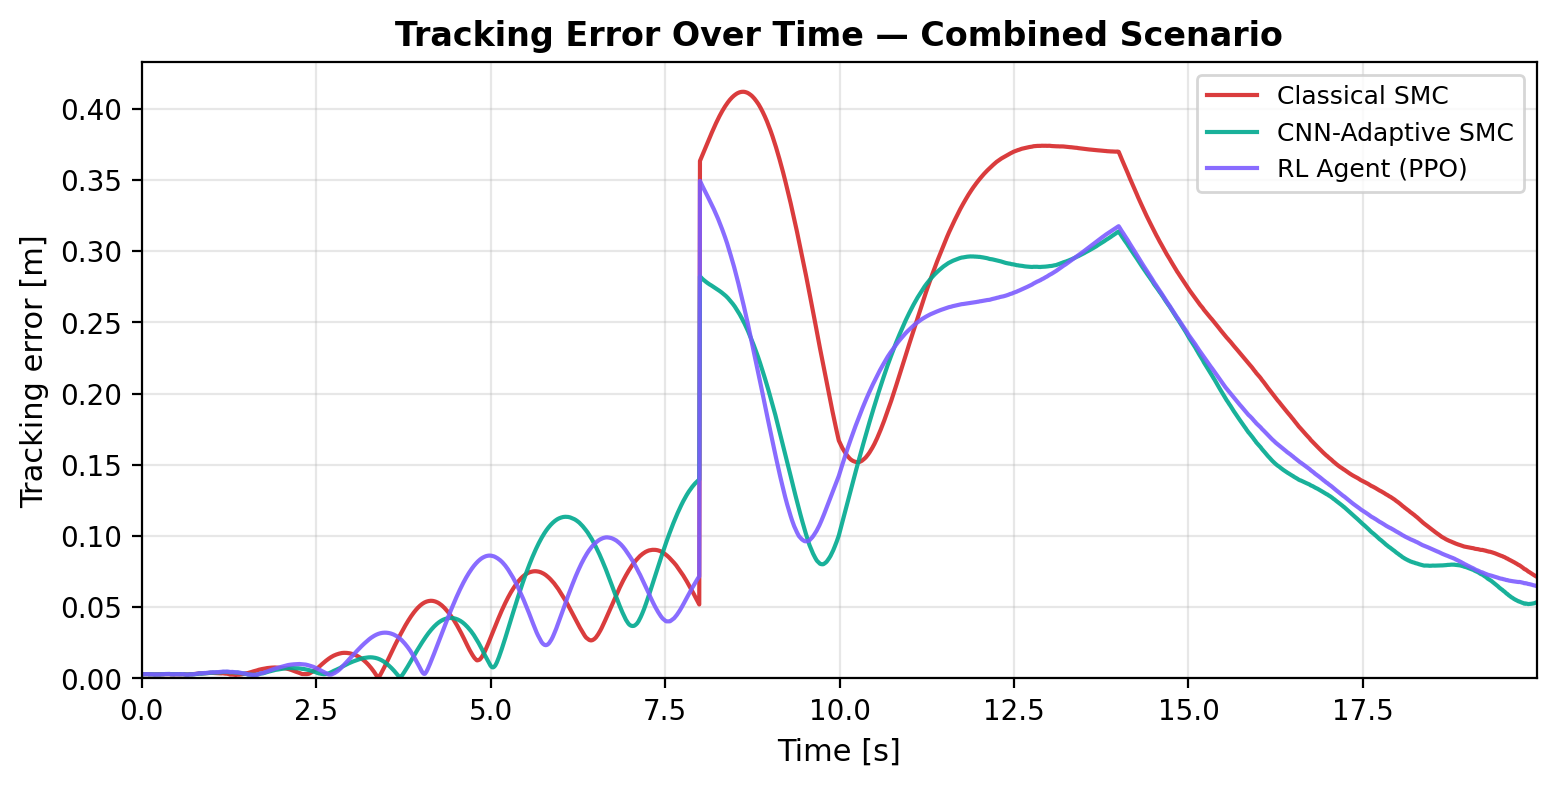
\includegraphics[width=0.82\textwidth]{../assets/figures/fig04_tracking_error.png}
  \end{center}
  \vspace{-0.15cm}
  {\small Full 20\,s episode: disturbance at $t=8$\,s, slip window $t\in[10,14]$\,s.}
\end{frame}

\begin{frame}{Quantitative Comparison}
  \begin{columns}[T]
    \begin{column}{0.48\textwidth}
      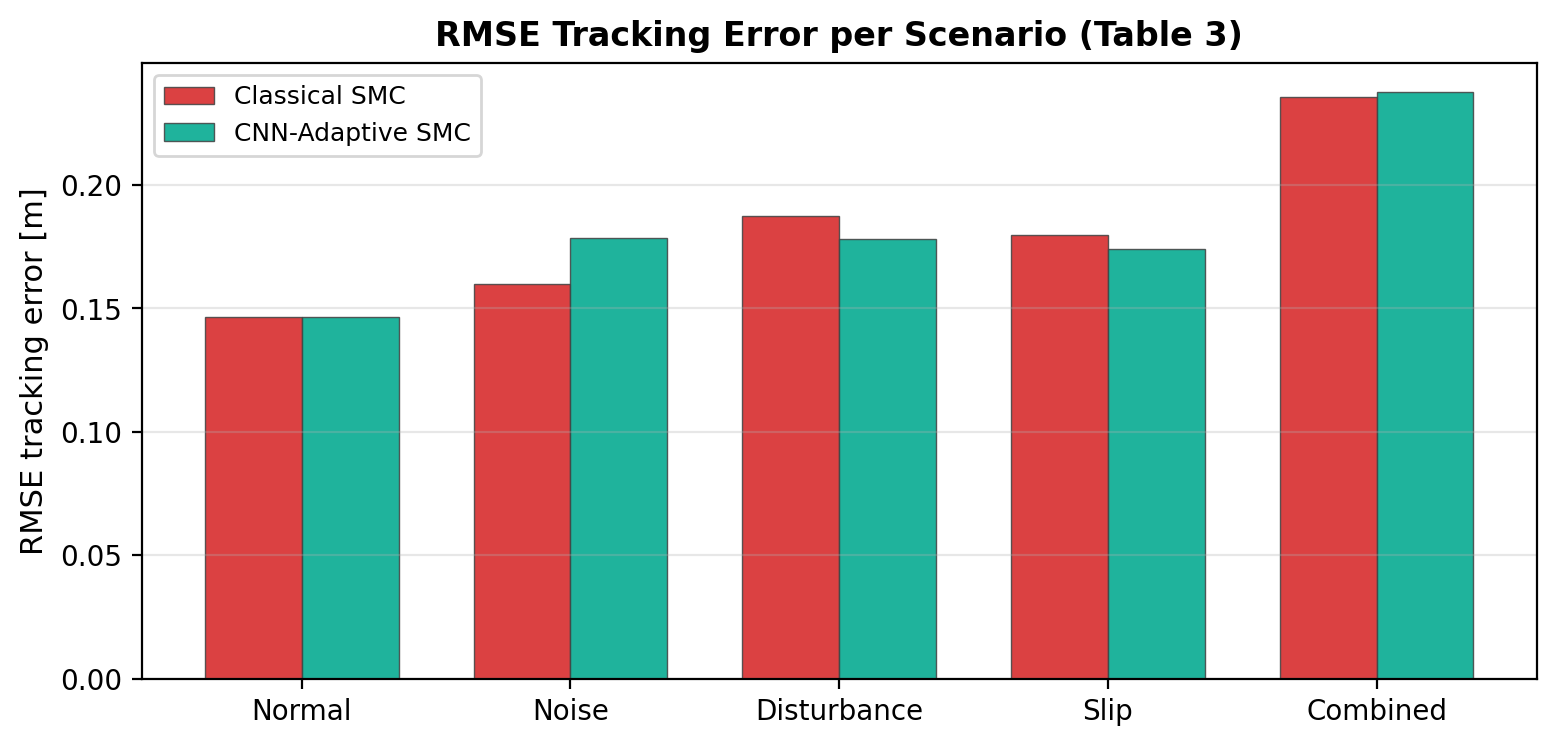
\includegraphics[width=\textwidth]{../assets/figures/fig05_rmse_bars.png}
    \end{column}
    \begin{column}{0.48\textwidth}
      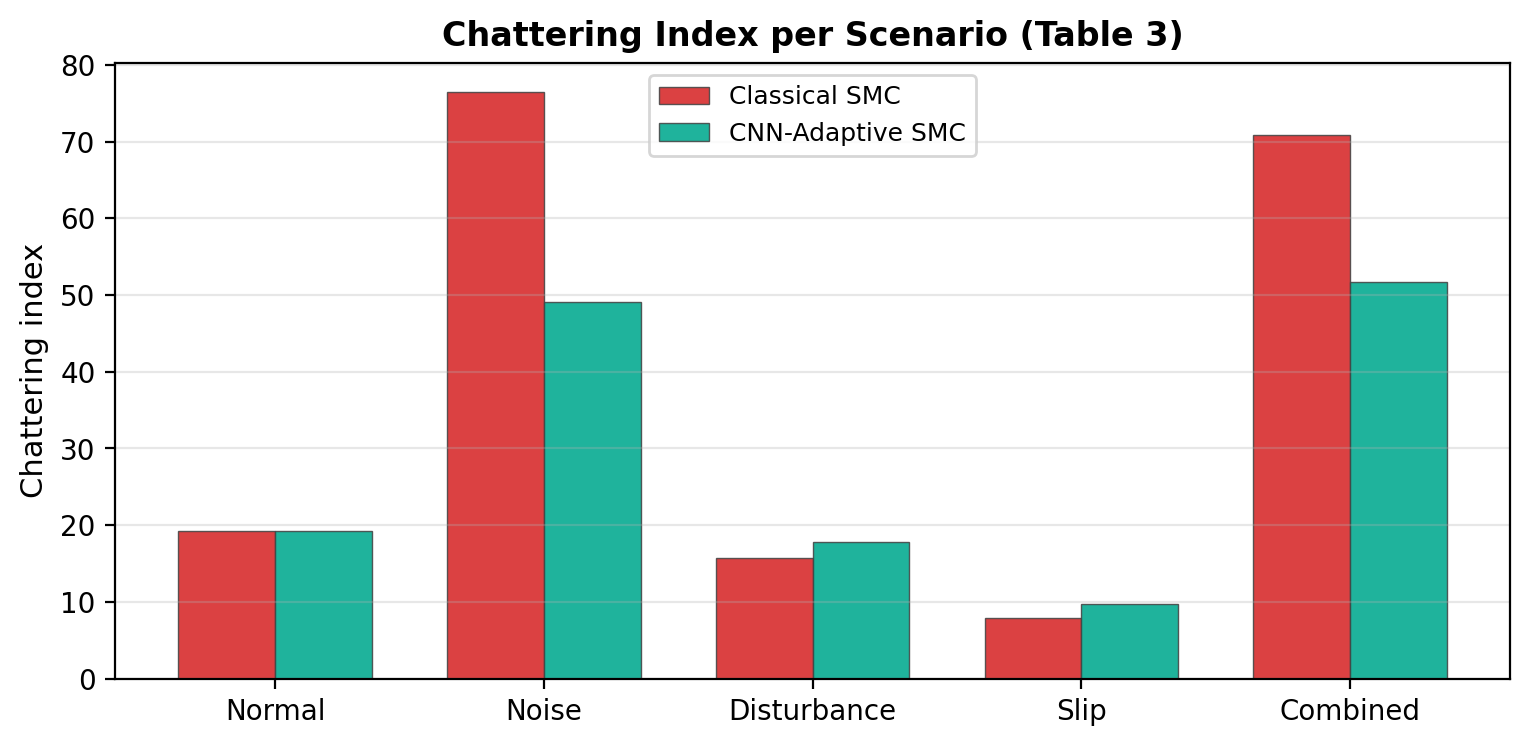
\includegraphics[width=\textwidth]{../assets/figures/fig06_chattering_bars.png}
    \end{column}
  \end{columns}
\end{frame}

\begin{frame}{Improvement Heatmap \& Multi-Controller Benchmark}
  \begin{columns}[T]
    \begin{column}{0.48\textwidth}
      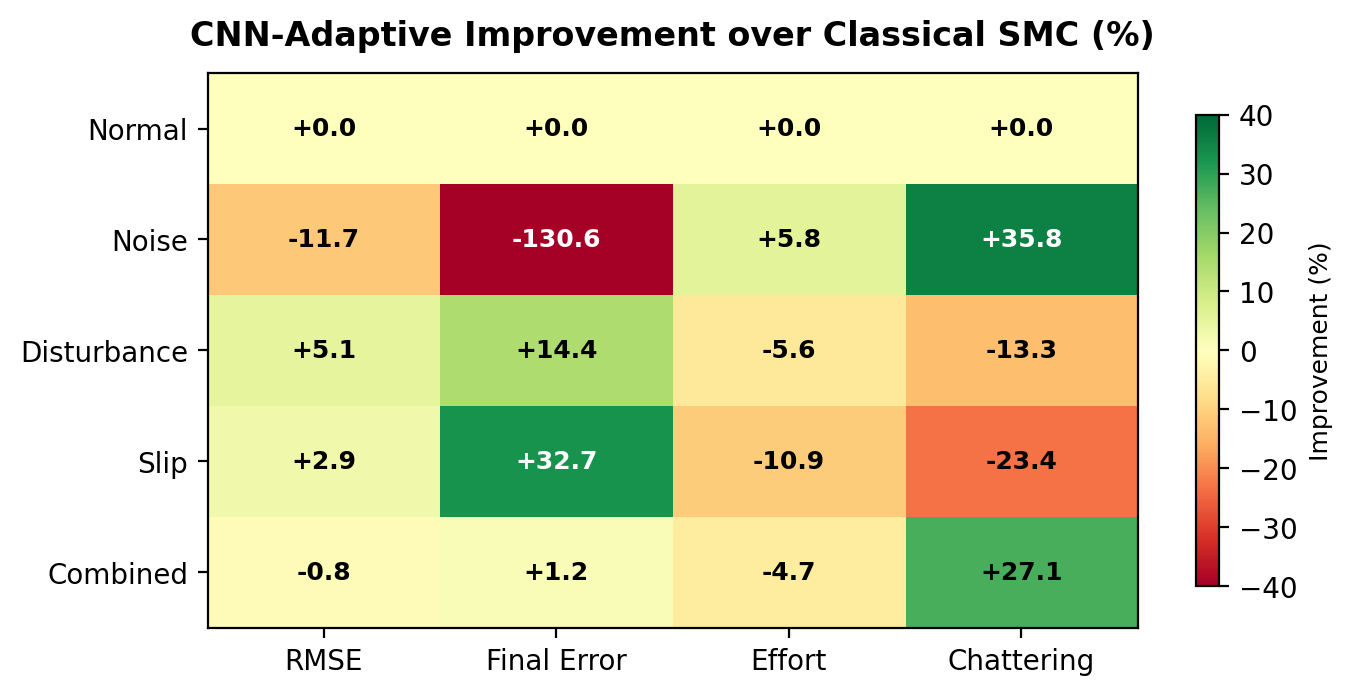
\includegraphics[width=\textwidth]{../assets/figures/fig09_improvement_heatmap.png}
    \end{column}
    \begin{column}{0.48\textwidth}
      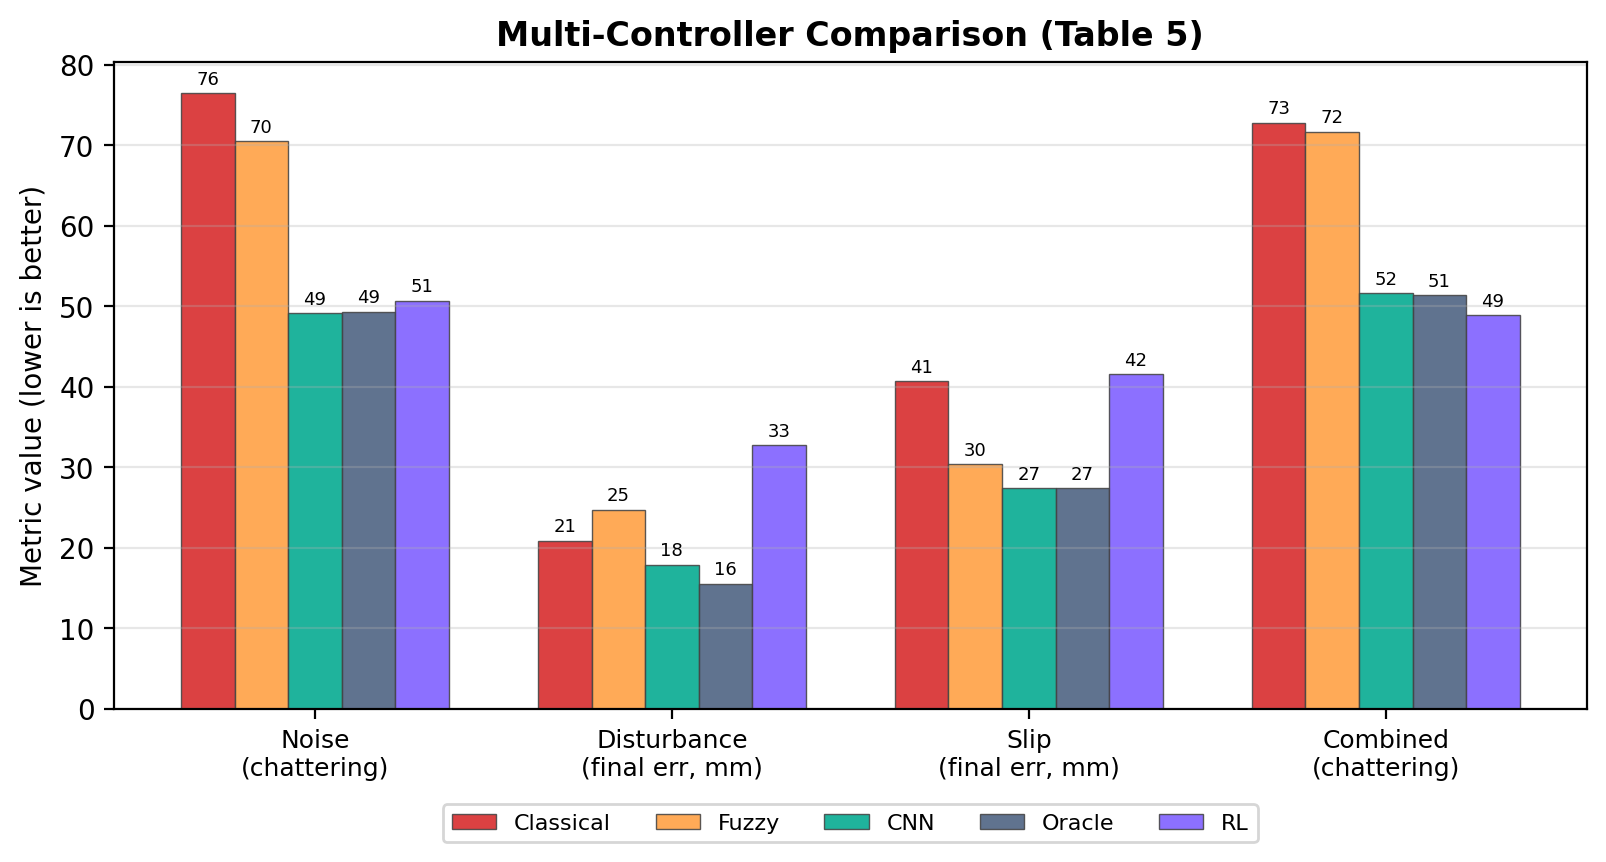
\includegraphics[width=\textwidth]{../assets/figures/fig10_multicontroller.png}
    \end{column}
  \end{columns}
  \vspace{0.2cm}
  {\small CNN-adaptive and oracle presets achieve largest chattering reductions; RL competitive under combined uncertainty.}
\end{frame}

\section{Digital Twin Demo}

\begin{frame}{Live Demonstration}
  \begin{columns}[T]
    \begin{column}{0.55\textwidth}
      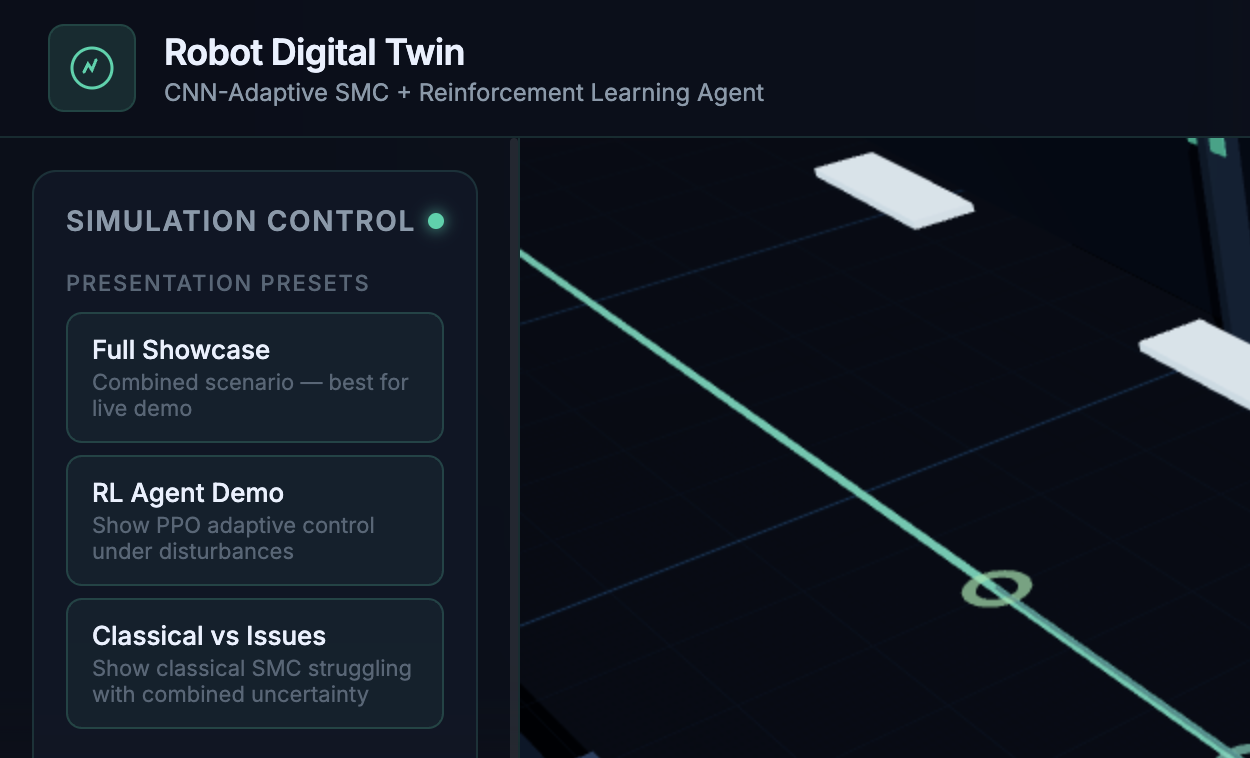
\includegraphics[width=\textwidth]{../assets/figures/fig08_digital_twin.png}
    \end{column}
    \begin{column}{0.43\textwidth}
      \textbf{Web-based 3D twin}
      \begin{itemize}
        \item React + Three.js frontend
        \item FastAPI WebSocket backend
        \item Hospital corridor environment
      \end{itemize}
      \vspace{0.3cm}
      \textbf{Demo flow}
      \begin{enumerate}
        \item \texttt{python run\_digital\_twin.py}
        \item Open \texttt{localhost:8000}
        \item Press \textbf{T} --- Controller Tour
        \item Compare tab --- benchmark
      \end{enumerate}
      \vspace{0.2cm}
      {\small Space = run/pause \quad 1/2/3 = controllers}
    \end{column}
  \end{columns}
\end{frame}

\section{Conclusion}

\begin{frame}{Conclusions}
  \begin{itemize}
    \item Complete pipeline: synthetic maps $\rightarrow$ CNN $\rightarrow$ adaptive SMC $\rightarrow$ simulation $\rightarrow$ digital twin.
    \item CNN-adaptive SMC \highlight{reduces chattering} and \highlight{improves recovery} with interpretable presets.
    \item Near-oracle performance vs.\ fuzzy and RL baselines on published benchmark.
    \item Lyapunov UUB analysis provides theoretical grounding for scenario-specific $\varphi$.
    \item Real-time 3D twin enables live defense demonstration.
  \end{itemize}
\end{frame}

\begin{frame}{Future Work \& Acknowledgement}
  \begin{columns}[T]
    \begin{column}{0.55\textwidth}
      \textbf{Future work}
      \begin{itemize}
        \item Real LiDAR occupancy grids
        \item Continuous on-line scenario inference
        \item Extended RL training + reward shaping
        \item Monte-Carlo evaluation + physical robot
      \end{itemize}
    \end{column}
    \begin{column}{0.42\textwidth}
      \textbf{Resources}
      \begin{itemize}
        \item Code: \url{github.com/LikhitaYerra/smc_cnn}
        \item Report: AI Clinic submission
        \item Conference: DELCON 2026
      \end{itemize}
      \vspace{0.5cm}
      \small We thank \textbf{aivancity} and Prof.\ Vishvjit Thakar for supervision and support.
    \end{column}
  \end{columns}
\end{frame}

\begin{frame}[plain,c]
  \begin{center}
    \vspace{1.5cm}
    {\Huge\bfseries\color{aivblue} Thank You}\\[0.8cm]
    {\Large Questions?}\\[1.2cm]
    
\includegraphics[height=1.2cm]{../assets/aivancity_logo.png}\\[0.6cm]
    {\small PGE5 --- AI Clinic \quad|\quad aivancity, Paris}
  \end{center}
\end{frame}

\end{document}
